\chapter{\textbf{Thông tin dự án}}
\label{sec:Bai1}

%======================
\section{Ngữ cảnh mô hình triển khai Printer Server}
%======================

\subsection{Chi tiết dự án}
\begin{table}[htbp]
\centering
\small
\begin{tabular}{|l|p{10.5cm}|}
\hline
\textbf{Nội dung} & \textbf{Chi tiết} \\
\hline
Tên Dự Án & Triển khai Printer Server – Doanh Nghiệp ABC \\
\hline
Môn học & Quản trị Hệ Thống Mạng \\
\hline
Ngôn Ngữ & Vietnamese/English \\
\hline
Phiên Bản & 1.0 – Production Ready \\
\hline
Ngày Hoàn Thành & November 2025 \\
\hline
Công Nghệ & Windows Server 2019, PowerShell, Active Directory \\
\hline
Yêu Cầu Đặc Biệt & Triển khai hoàn toàn qua dòng lệnh – Không dùng GUI \\
\hline
\end{tabular}
\caption{Thông tin tổng quan dự án}
\label{tab:project_info}
\end{table}

\subsection{Bối cảnh doanh nghiệp ABC}

Doanh nghiệp có 3 phòng ban, mỗi phòng có yêu cầu in ấn khác nhau:

\begin{itemize}[leftmargin=*,noitemsep,topsep=3pt]
    \item \textbf{Phòng Thiết kế (Design):} cần in màu chất lượng cao, ưu tiên tốc độ.
    \item \textbf{Phòng Văn phòng (Office):} in văn bản số lượng lớn, ưu tiên tiết kiệm chi phí.
    \item \textbf{Phòng Kế toán (Accounting):} in hóa đơn, yêu cầu bảo mật cao và ghi log chi tiết.
\end{itemize}

\noindent\textbf{Yêu cầu hệ thống:}
\begin{itemize}[leftmargin=*,noitemsep,topsep=3pt]
    \item Mỗi phòng ban chỉ được truy cập đúng máy in phụ trách.
    \item Tự động phân phối máy in qua Group Policy (client tự nhận máy in khi đăng nhập).
    \item Tạo Printer Pool để chia tải giữa các máy in.
    \item Quản lý và phân quyền in theo user/group trong AD.
    \item Ghi log chi tiết nhật ký in: thời gian, user, số trang, tên tài liệu.
    \item Xuất báo cáo thống kê phục vụ audit và giám sát.
\end{itemize}

\subsection{Mục tiêu}
\begin{itemize}[leftmargin=*,noitemsep,topsep=3pt]
    \item Tự động hóa triển khai, phân phối và giám sát máy in bằng PowerShell.
    \item Minh họa đầy đủ cấu hình AD, GPO, Print Server, Printer Pool và phân quyền.
    \item Xây dựng hệ thống mô phỏng sát thực tế doanh nghiệp: ổn định – bảo mật – tự động.
\end{itemize}
\vspace{\baselineskip}
\vspace{\baselineskip}

\chapter{\textbf{Hạ tầng hệ thống}}

\section{Cấu hình máy chủ Print Server}

\begin{figure}[htbp]
    \centering
    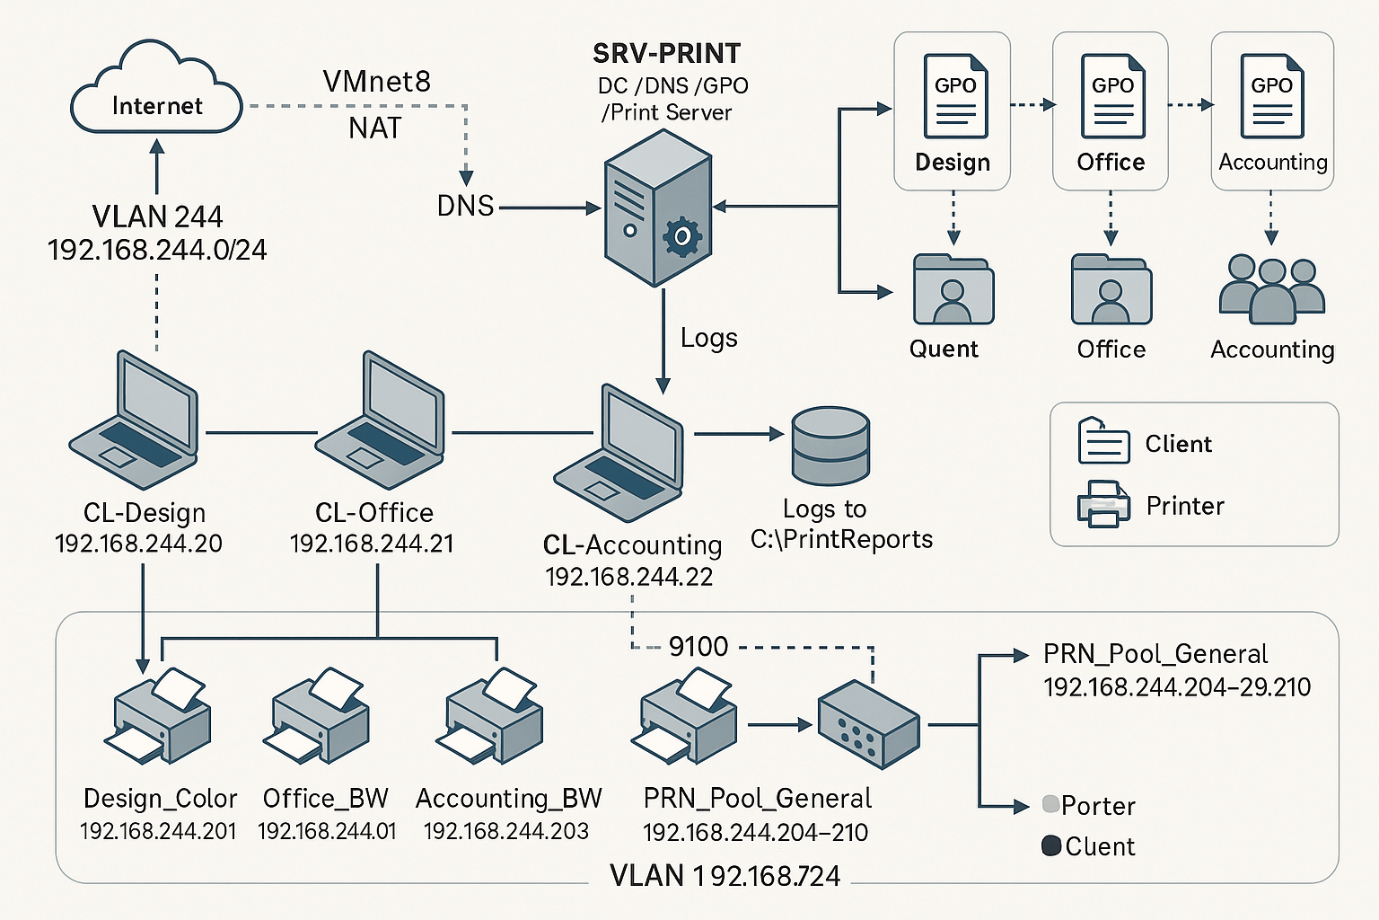
\includegraphics[width=0.92\linewidth]{./media/Sơ đồ cấu trúc hệ thống.png}
    \caption{Sơ đồ cấu trúc tổng thể hệ thống Printer Server}
    \label{fig:system_architecture}
\end{figure}

\subsection{Mô tả thành phần trong kiến trúc}

\begin{itemize}[leftmargin=*,noitemsep,topsep=3pt]
    \item \textbf{1 máy chủ Windows Server 2019 (VMware):}
    \begin{itemize}[noitemsep]
        \item Cài đặt các vai trò: \textbf{Print Server}, \textbf{Active Directory Domain Services}, \textbf{DNS}.
        \item Tham gia domain: \textbf{ABC.local}.
        \item Đóng vai trò máy chủ chính cung cấp dịch vụ in, phân phối máy in và lưu log.
    \end{itemize}

    \item \textbf{3 máy trạm Windows 8.1:}
    \begin{itemize}[noitemsep]
        \item Đại diện cho 3 người dùng thuộc 3 phòng ban: \textit{user\_design}, \textit{user\_office}, \textit{user\_accounting}.
        \item Các máy này nhận máy in tự động thông qua Group Policy.
    \end{itemize}

    \item \textbf{10 máy in vật lý/ảo:}
    \begin{itemize}[noitemsep]
        \item Dải IP sử dụng: \textbf{192.168.244.201 – 192.168.244.210}.
        \item Bao gồm máy in màu, máy in trắng đen và máy in hoá đơn theo nhu cầu từng phòng ban.
    \end{itemize}
\end{itemize}

\begin{table}[htbp]
\centering
\small
\begin{tabular}{|l|p{10.5cm}|}
\hline
\textbf{Thông số} & \textbf{Chi tiết} \\
\hline
Hostname & SRV-PRINT \\
\hline
OS & Windows Server 2019 Datacenter \\
\hline
IP Address & 192.168.244.10/24 \\
\hline
Gateway & 192.168.244.1 \\
\hline
DNS Primary & 192.168.244.10 \\
\hline
DNS Secondary & 8.8.8.8 \\
\hline
Domain & ABC.local \\
\hline
Vai trò & DC + Print Server + DNS + AD DS \\
\hline
Nền tảng & VMware Workstation Pro (Bridged) \\
\hline
\end{tabular}
\caption{Thông số cấu hình Print Server}
\label{tab:print_server_config}
\end{table}

\noindent\textbf{Tóm tắt cấu hình mạng:}
\begin{itemize}[leftmargin=*,noitemsep,topsep=3pt]
    \item \textbf{Server:} Windows Server 2019 (VMware), IP: \textbf{192.168.244.10/24}, Gateway: \textbf{192.168.244.1}.
    \item \textbf{Domain:} \textbf{ABC.local}, tên máy chủ: \textbf{SRV-PRINT}.
    \item \textbf{Client:} Windows 8.1 (đã join domain ABC.local), IP thuộc dải \textbf{192.168.244.x}.
    \item \textbf{Máy in:} các máy in vật lý/ảo sử dụng dải IP \textbf{192.168.244.201–210}.
\end{itemize}

\subsection{Sơ đồ hoạt động hệ thống}
\begin{figure}[htbp]
    \centering
    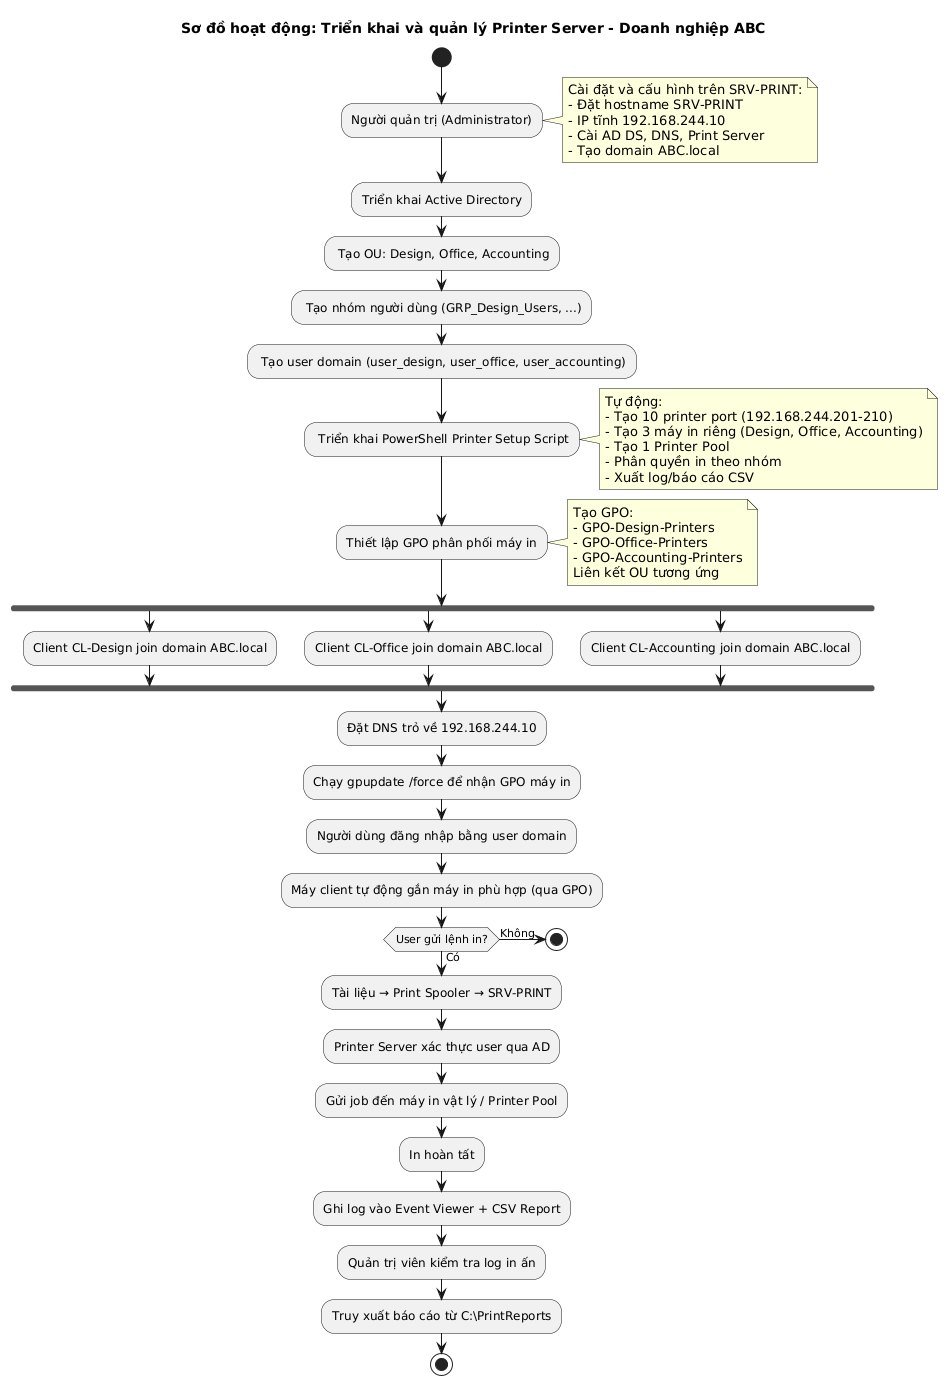
\includegraphics[width=0.88\linewidth]{./media/Sơ đồ hoạt động.png}
    \caption{Sơ đồ hoạt động của hệ thống Printer Server}
    \label{fig:system_flow}
\end{figure}

\section{Cấu trúc Active Directory}
\begin{figure}[htbp]
    \centering
    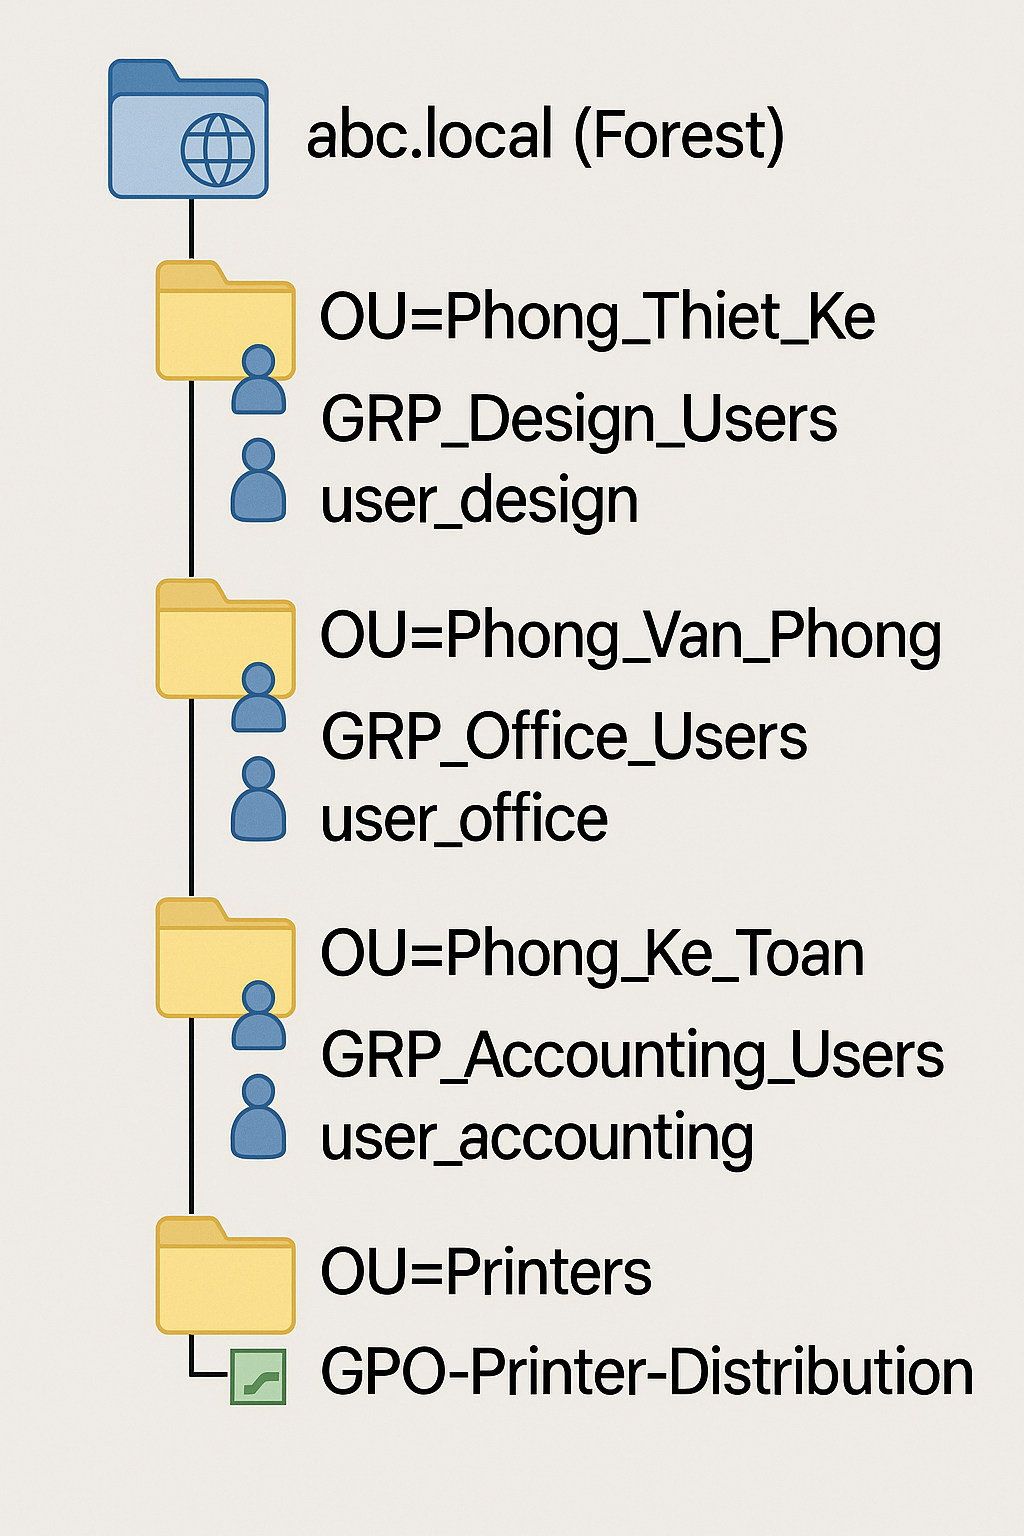
\includegraphics[width=0.72\linewidth]{./media/Cấu trúc Active Directory.png}
    \caption{Cấu trúc Active Directory}
    \label{fig:ad_structure}
\end{figure}

\section{Dải IP và các Port}
\begin{table}[htbp]
\centering
\small
\caption{Phân bổ địa chỉ IP trong mô hình triển khai}
\label{tab:ip-allocation}
\begin{tabular}{|p{2.8cm}|p{2.8cm}|p{3.2cm}|p{4.8cm}|}
\hline
\textbf{Loại thiết bị} & \textbf{Dải IP} & \textbf{Địa chỉ cụ thể} & \textbf{Mục đích sử dụng} \\ \hline
Server & 192.168.244.10/24 & 192.168.244.10 & Máy chủ Print Server (SRV-PRINT) - Windows Server 2019 trên VMware \\ \hline
Gateway & 192.168.244.1 & 192.168.244.1 & Cổng mạng mặc định cho toàn bộ hệ thống \\ \hline
Client computers & 192.168.244.20-99 & 192.168.244.20 \newline 192.168.244.21 \newline 192.168.244.x & Máy trạm Windows 8.1 đã join domain: \newline - user\_design (Phòng Thiết kế) \newline - user\_office (Phòng Văn phòng) \newline - user\_accounting (Phòng Kế toán) \\ \hline
Máy in vật lý/ảo & 192.168.244.201-210 & 192.168.244.201 \newline 192.168.244.202 \newline 192.168.244.203 \newline ... \newline 192.168.244.210 & 10 máy in được phân bổ cho các phòng ban: \newline - Máy in màu cao cấp (Phòng Thiết kế) \newline - Máy in laser trắng đen (Phòng Văn phòng) \newline - Máy in bảo mật (Phòng Kế toán) \newline - Các máy in dự phòng/Printer Pool \\ \hline
\end{tabular}
\end{table}

\subsection*{Thông tin Subnet}
\begin{itemize}[leftmargin=*,noitemsep,topsep=3pt]
    \item \textbf{Subnet Mask:} 255.255.255.0 (/24)
    \item \textbf{Network Address:} 192.168.244.0
    \item \textbf{Broadcast Address:} 192.168.244.255
    \item \textbf{Số IP khả dụng:} 254 địa chỉ (192.168.244.1 - 192.168.244.254)
\end{itemize}

\subsection*{Phân vùng IP đề xuất}
\begin{itemize}[leftmargin=*,noitemsep,topsep=3pt]
    \item \textbf{192.168.244.1-9:} Thiết bị mạng (Gateway, Switch, Router)
    \item \textbf{192.168.244.10-19:} Servers (Domain Controller, Print Server, File Server...)
    \item \textbf{192.168.244.20-199:} Client computers (máy trạm người dùng)
    \item \textbf{192.168.244.200-254:} Thiết bị ngoại vi (Máy in, Scanner, Thiết bị IoT)
\end{itemize}
\vspace{\baselineskip}
\chapter{\textbf{Các bước chuẩn bị}}
\section{Thiết lập Hostname, IP tĩnh trên Server}

\begin{lstlisting}[style=powershell]
# 0.1 Set Hostname = SRV-PRINT
$NewHostname = "SRV-PRINT" 
$CurrentHostname = $env:COMPUTERNAME

if ($CurrentHostname -ne $NewHostname) {
    Write-Host "Changing hostname from $CurrentHostname -> $NewHostname" -ForegroundColor Cyan
    Rename-Computer -NewName $NewHostname -Force
    Write-Host "[OK] Hostname will change after restart" -ForegroundColor Green
} else {
    Write-Host "Hostname is already SRV-PRINT" -ForegroundColor Green
}

# 0.2 Static IP Configuration: 192.168.244.10/24, Gateway: 192.168.244.1
Write-Host "--- Static IP Configuration ---" -ForegroundColor Cyan

$IPAddress = "192.168.244.10" 
$SubnetMask = "255.255.255.0" 
$Gateway = "192.168.244.1" 
$DNS = @("8.8.8.8", "8.8.4.4") # Temporary DNS, DC will be used as DNS later

# Get Ethernet adapter
$NetworkAdapter = Get-NetAdapter | Where-Object {$_.Status -eq "Up"} | Select-Object -First 1

if ($NetworkAdapter) {
    Write-Host "Adapter found: $($NetworkAdapter.Name)" -ForegroundColor Green
    
    # Remove old DHCP configuration
    try {
        Remove-NetIPAddress -InterfaceAlias $NetworkAdapter.Name -Confirm:$false -ErrorAction SilentlyContinue
        Remove-NetRoute -InterfaceAlias $NetworkAdapter.Name -Confirm:$false -ErrorAction SilentlyContinue
    } catch {
        Write-Host " Error removing old configuration: $_" -ForegroundColor Yellow
    }

    # Set Static IP
    try {
        New-NetIPAddress -InterfaceAlias $NetworkAdapter.Name `
            -IPAddress $IPAddress `
            -PrefixLength 24 `
            -DefaultGateway $Gateway `
            -AddressFamily IPv4 `
            -ErrorAction Stop
        Write-Host " IP $IPAddress set successfully" -ForegroundColor Green
    } catch {
        Write-Host " Error setting IP: $_" -ForegroundColor Yellow
    }

    # Set DNS
    try {
        Set-DnsClientServerAddress -InterfaceAlias $NetworkAdapter.Name `
            -ServerAddresses $DNS `
            -ErrorAction Stop
        Write-Host " DNS set successfully" -ForegroundColor Green
    } catch {
        Write-Host " Error setting DNS: $_" -ForegroundColor Yellow
    }

} else {
    Write-Host " Network Adapter not found" -ForegroundColor Red
}

# Verify network configuration
Write-Host "--- Verify Network Configuration ---" -ForegroundColor Cyan
Get-NetIPAddress -AddressFamily IPv4 | Format-Table -AutoSize
Get-DnsClientServerAddress -AddressFamily IPv4 | Format-Table -AutoSize
\end{lstlisting}

\begin{table}[htbp]
\centering
\small
\begin{tabular}{|p{5cm}|p{6cm}|}
\hline
\textbf{Biến} & \textbf{Giá trị} \\
\hline
\texttt{\$IPAddress} & "192.168.244.10" \\
\hline
\texttt{\$SubnetMask} & "255.255.255.0" \\
\hline
\texttt{\$Gateway} & "192.168.244.1" \\
\hline
\texttt{\$DNS1} & "192.168.244.10" \\
\hline
\texttt{\$DNS2} & "8.8.8.8" \\
\hline
\end{tabular}
\caption{Cấu hình IP Static}
\label{tab:ip_static}
\end{table}

\begin{figure}[htbp]
    \centering
    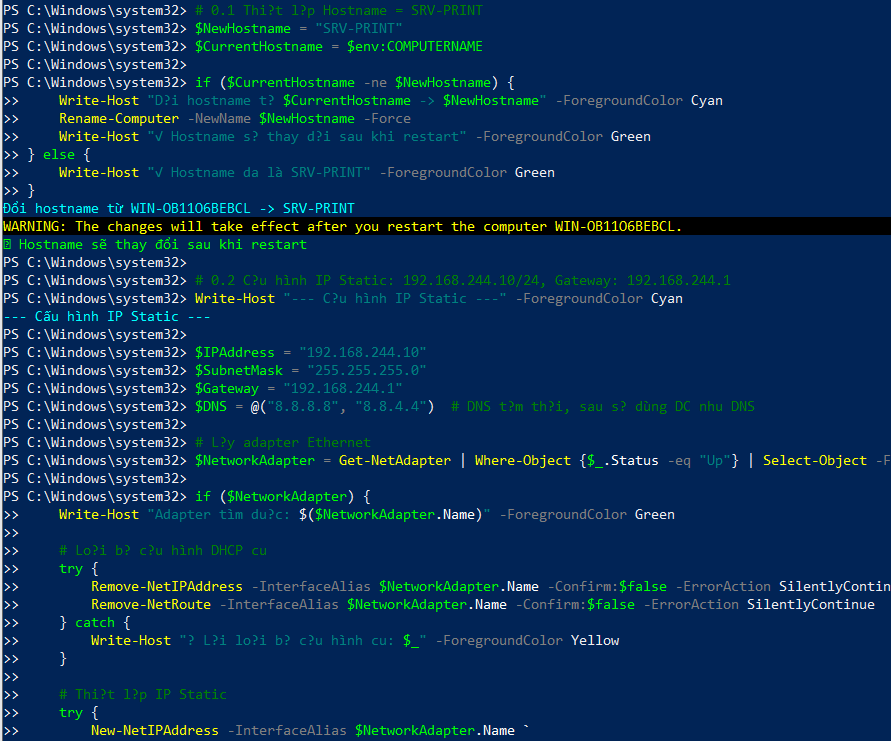
\includegraphics[width=0.78\linewidth]{./media/CẤU HÌNH BAN ĐẦU (HOSTNAME, IP, NETWORK).png}
    \caption{Cấu hình ban đầu}
    \label{fig:initial_config}
\end{figure}

\begin{figure}[htbp]
    \centering
    \begin{minipage}[b]{0.48\textwidth}
        \centering
        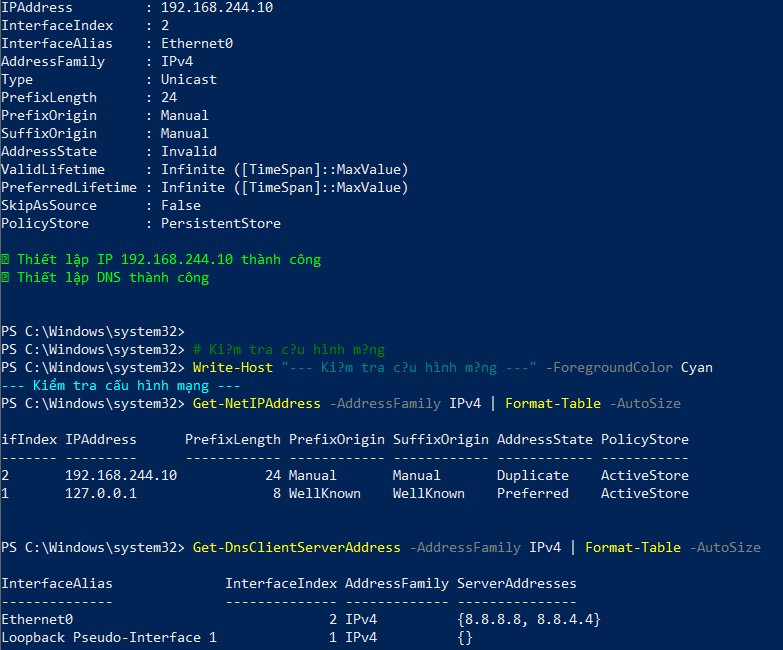
\includegraphics[width=\textwidth]{./media/Thiết lập ip static(1).png}
        \caption{Thiết lập IP static (1)}
        \label{fig:ip_static1}
    \end{minipage}
    \hfill
    \begin{minipage}[b]{0.48\textwidth}
        \centering
        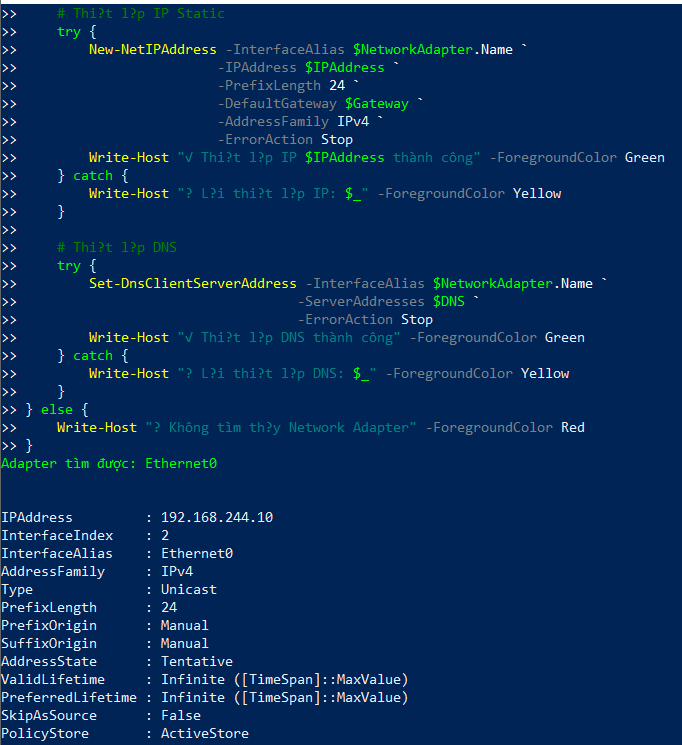
\includegraphics[width=\textwidth]{./media/Thiết lập ip static.png}
        \caption{Thiết lập IP static (2)}
        \label{fig:ip_static2}
    \end{minipage}
\end{figure}

\section{Cài đặt Server, AD, DS, DNS}
\subsection{Cấu hình ban đầu trên Server (Windows Server 2019)}

\begin{lstlisting}[style=powershell]
# 1.1 Install Print and Document Services Role
Write-Host "=== STEP 1: Install Print Server Role ===" -ForegroundColor Cyan
Install-WindowsFeature -Name Print-Server -IncludeManagementTools -Restart:$false
Write-Host "[OK] Print Server installed" -ForegroundColor Green

# 1.2 Check Print Server status
Get-WindowsFeature -Name Print-Server | Select-Object Name, Installed

# 1.3 Start Print Spooler service
Write-Host "=== STEP 2: Start Print Spooler service ===" -ForegroundColor Cyan
Start-Service -Name Spooler
Set-Service -Name Spooler -StartupType Automatic
Get-Service -Name Spooler
\end{lstlisting}

\begin{figure}[htbp]
    \centering
    \begin{minipage}[b]{0.48\textwidth}
        \centering
        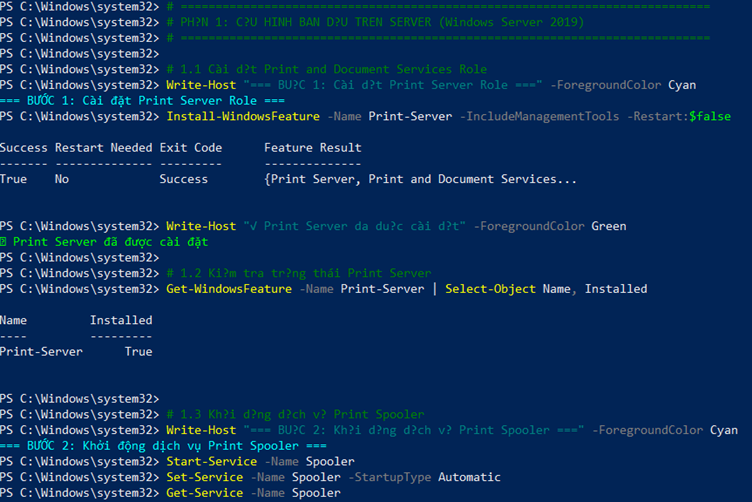
\includegraphics[width=\textwidth]{./media/CH Ban Đầu.png}
        \caption{Cấu hình ban đầu (1)}
        \label{fig:config_initial1}
    \end{minipage}
    \hfill
    \begin{minipage}[b]{0.48\textwidth}
        \centering
        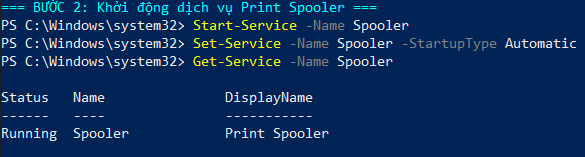
\includegraphics[width=\textwidth]{./media/Cấu hình winserv2019(1).png}
        \caption{Cấu hình ban đầu (2)}
        \label{fig:config_initial2}
    \end{minipage}
\end{figure}

\subsection{Cài đặt Active Directory Domain Controller}

\begin{lstlisting}[style=powershell]
# 1.1 Install AD DS Role
try {
    Install-WindowsFeature -Name AD-Domain-Services -IncludeManagementTools -Restart:$false -ErrorAction Stop
    Write-Host "[OK] AD Domain Services installed" -ForegroundColor Green
} catch {
    Write-Host "[!] AD DS installed or error: $_" -ForegroundColor Yellow
}

# 1.2 Install DNS Server (required for DC)
try {
    Install-WindowsFeature -Name DNS -IncludeManagementTools -Restart:$false -ErrorAction Stop
    Write-Host "[OK] DNS Server installed" -ForegroundColor Green
} catch {
    Write-Host "[!] DNS Server installed or error: $_" -ForegroundColor Yellow
}

# 1.3 Create Forest and Domain: ABC.local
Write-Host "--- Create Domain ABC.local ---" -ForegroundColor Cyan
$DomainName = "ABC.local" 
$SafeModePW = ConvertTo-SecureString -AsPlainText "Manh31102005" -Force

try {
    Install-ADDSForest -DomainName $DomainName `
    -SafeModeAdministratorPassword $SafeModePW `
    -InstallDNS `
    -NoRebootOnCompletion:$false `
    -Force `
    -WarningAction SilentlyContinue `
    -ErrorAction Stop
    
    Write-Host "[OK] Domain $DomainName created successfully" -ForegroundColor Green
    Write-Host "[OK] Server will automatically restart to complete setup" -ForegroundColor Green
    Start-Sleep -Seconds 5
}
catch {
    Write-Host "[!] Error creating Domain: $_" -ForegroundColor Yellow
}
\end{lstlisting}

\begin{figure}[htbp]
    \centering
    \begin{minipage}[b]{0.48\textwidth}
        \centering
        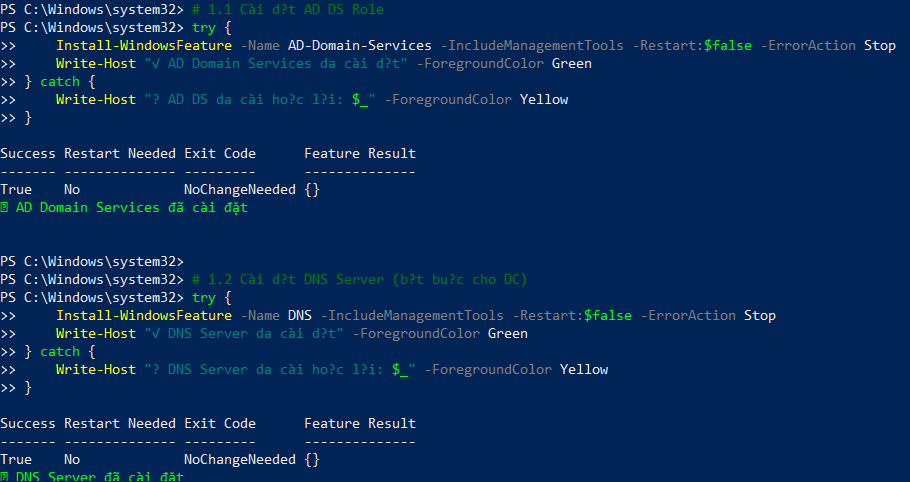
\includegraphics[width=\textwidth]{./media/Cài đặt AD DS role.png}
        \caption{Cài đặt AD DS role (1)}
        \label{fig:adds_install1}
    \end{minipage}
    \hfill
    \begin{minipage}[b]{0.48\textwidth}
        \centering
        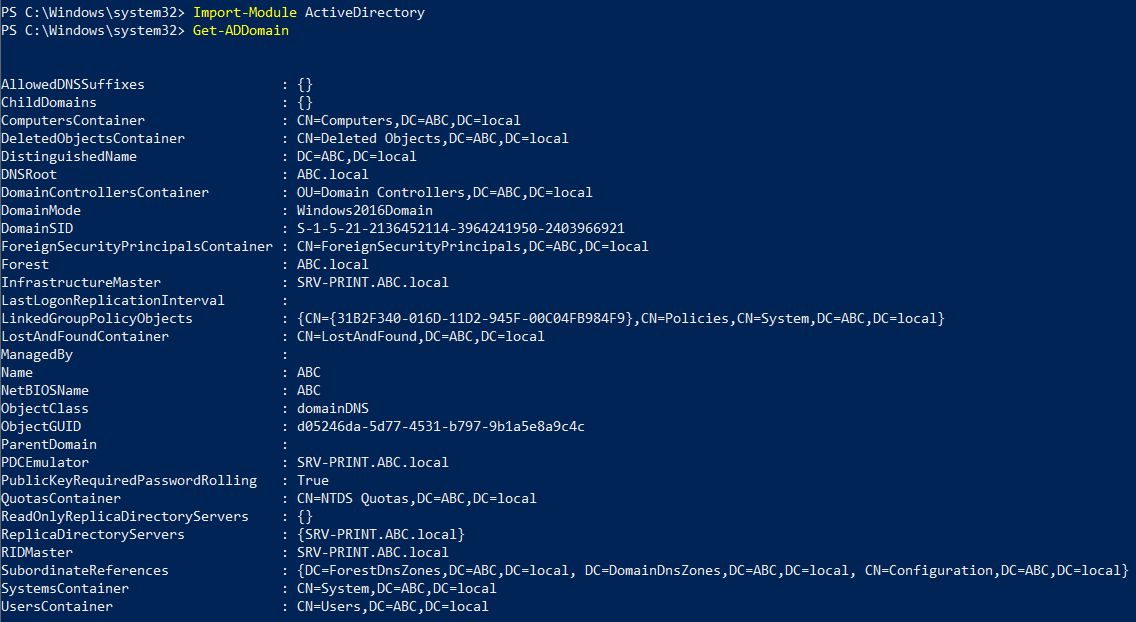
\includegraphics[width=\textwidth]{./media/Cài đặt AD DS role(1).png}
        \caption{Cài đặt AD DS role (2)}
        \label{fig:adds_install2}
    \end{minipage}
\end{figure}

\section{Tạo cấu trúc nhóm Active Directory}

\textbf{Tạo nhóm AD cho từng phòng ban}

\begin{itemize}[leftmargin=*,noitemsep,topsep=3pt]
    \item \textbf{Cài RSAT-AD-PowerShell (module ActiveDirectory)}
\end{itemize}

\begin{lstlisting}[style=powershell]
Install-WindowsFeature AD-Domain-Services, RSAT-AD-PowerShell -IncludeManagementTools
\end{lstlisting}

\begin{figure}[htbp]
    \centering
    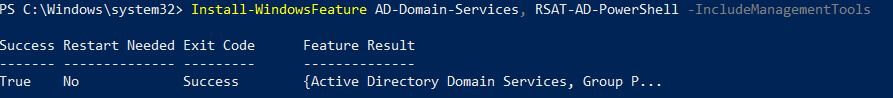
\includegraphics[width=0.72\linewidth]{./media/Cài RSAT-AD-PowerShell (module ActiveDirectory).png}
    \caption{Cài RSAT-AD-PowerShell}
    \label{fig:rsat_install}
\end{figure}

\begin{itemize}[leftmargin=*,noitemsep,topsep=3pt]
    \item \textbf{Tạo Nhóm AD cho từng phòng ban}
\end{itemize}

\begin{lstlisting}[style=powershell]
$DomainDN = "DC=ABC,DC=local" 
$OUPath = "OU=PrinterGroups,OU=PrinterManagement,$DomainDN" 
$UserOUPath = "OU=Users,OU=PrinterManagement,$DomainDN" 

Write-Host "--- Create Test Users ---" -ForegroundColor Cyan

$Password = ConvertTo-SecureString -AsPlainText "Manh31102005" -Force

$Users = @(
    @{
        UserName="user_design"
        GivenName="User"
        Surname="Design"
        GroupName="GRP_Design"
        Description="Design Department User"
    }, 
    @{
        UserName="user_office"
        GivenName="User"
        Surname="Office"
        GroupName="GRP_Office"
        Description="Office Department User"
    }, 
    @{
        UserName="user_accounting"
        GivenName="User"
        Surname="Accounting"
        GroupName="GRP_Accounting"
        Description="Accounting Department User"
    }
)

foreach ($user in $Users) {
    try {
        New-ADUser -SamAccountName $user.UserName `
            -UserPrincipalName "$($user.UserName)@ABC.local" `
            -GivenName $user.GivenName `
            -Surname $user.Surname `
            -Name "$($user.GivenName) $($user.Surname)" `
            -DisplayName "$($user.GivenName) $($user.Surname)" `
            -Description $user.Description `
            -AccountPassword $Password `
            -Enabled $true `
            -PasswordNeverExpires $true `
            -Path $UserOUPath `
            -ErrorAction Stop
            
        Write-Host "[OK] User '$($user.UserName)' created successfully" -ForegroundColor Green

        # Add user to corresponding group
        Add-ADGroupMember -Identity $user.GroupName -Members $user.UserName -ErrorAction Stop
        
        Write-Host " [OK] Added '$($user.UserName)' to group '$($user.GroupName)'" -ForegroundColor Green

    } catch {
        Write-Host "[!] Error with user '$($user.UserName)': $_" -ForegroundColor Yellow
    }
}
\end{lstlisting}

\begin{figure}[htbp]
    \centering
    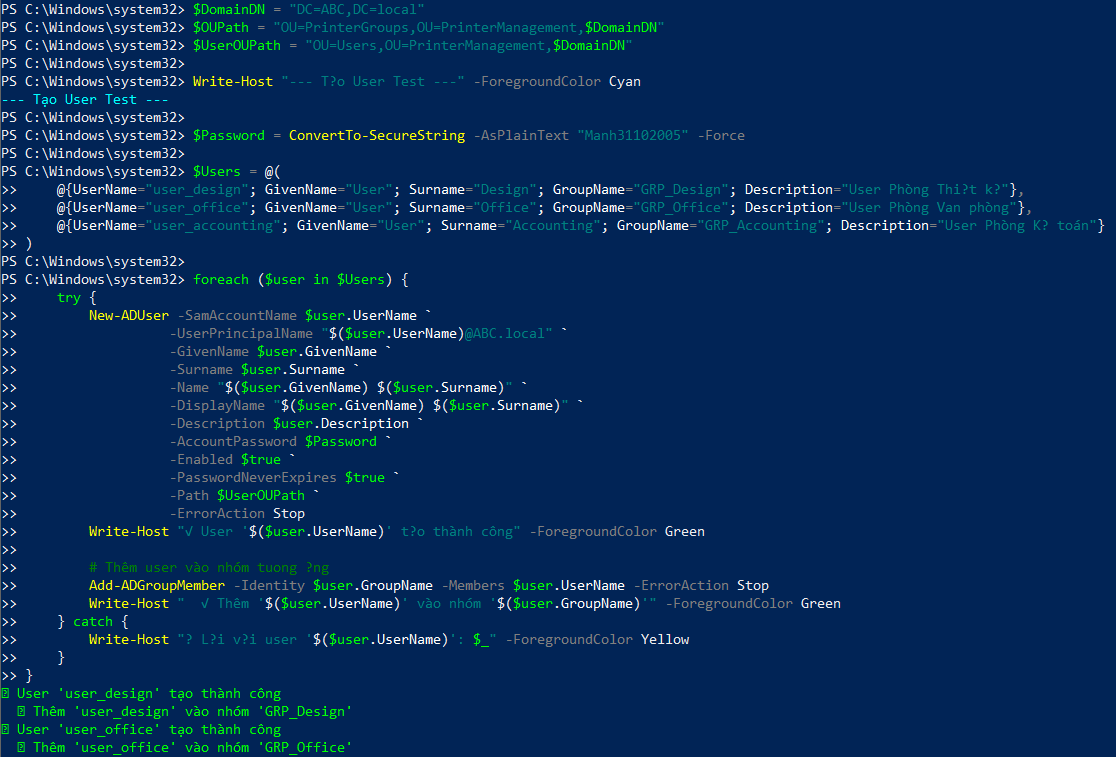
\includegraphics[width=0.78\textwidth]{./media/Tạo Nhóm AD cho từng phòng ban.png}
    \caption{Tạo Nhóm AD cho từng phòng ban}
    \label{fig:ad_groups}
\end{figure}

\chapter{\textbf{Tạo nhóm và người dùng}}
\section{Tạo nhóm theo từng phòng ban}

\begin{lstlisting}[style=powershell]
$DomainDN = "DC=ABC,DC=local"
$OUPath = "OU=PrinterGroups,OU=PrinterManagement,$DomainDN"
$UserOUPath = "OU=Users,OU=PrinterManagement,$DomainDN"

Write-Host "--- Tao User Test ---" -ForegroundColor Cyan

$Password = ConvertTo-SecureString -AsPlainText "Manh31102005" -Force

$Users = @(
    @{UserName="user_design"; GivenName="User"; Surname="Design"; GroupName="GRP_Design"; Description="User Phong Thiet ke"},
    @{UserName="user_office"; GivenName="User"; Surname="Office"; GroupName="GRP_Office"; Description="User Phong Van phong"},
    @{UserName="user_accounting"; GivenName="User"; Surname="Accounting"; GroupName="GRP_Accounting"; Description="User Phong Ke toan"}
)
\end{lstlisting}

\section{Tạo User tương ứng}

\begin{lstlisting}[style=powershell]
foreach ($user in $Users) {
    try {
        New-ADUser -SamAccountName $user.UserName `
                  -UserPrincipalName "$($user.UserName)@ABC.local" `
                  -GivenName $user.GivenName `
                  -Surname $user.Surname `
                  -Name "$($user.GivenName) $($user.Surname)" `
                  -DisplayName "$($user.GivenName) $($user.Surname)" `
                  -Description $user.Description `
                  -AccountPassword $Password `
                  -Enabled $true `
                  -PasswordNeverExpires $true `
                  -Path $UserOUPath `
                  -ErrorAction Stop
        Write-Host "[OK] User '$($user.UserName)' tao thanh cong" -ForegroundColor Green
        
        # Them user vao nhom tuong ung
        Add-ADGroupMember -Identity $user.GroupName -Members $user.UserName -ErrorAction Stop
        Write-Host " [OK] Them '$($user.UserName)' vao nhom '$($user.GroupName)'" -ForegroundColor Green
    } catch {
        Write-Host "[!] Loi voi user '$($user.UserName)': $_" -ForegroundColor Yellow
    }
}
\end{lstlisting}

\begin{figure}[htbp]
    \centering
    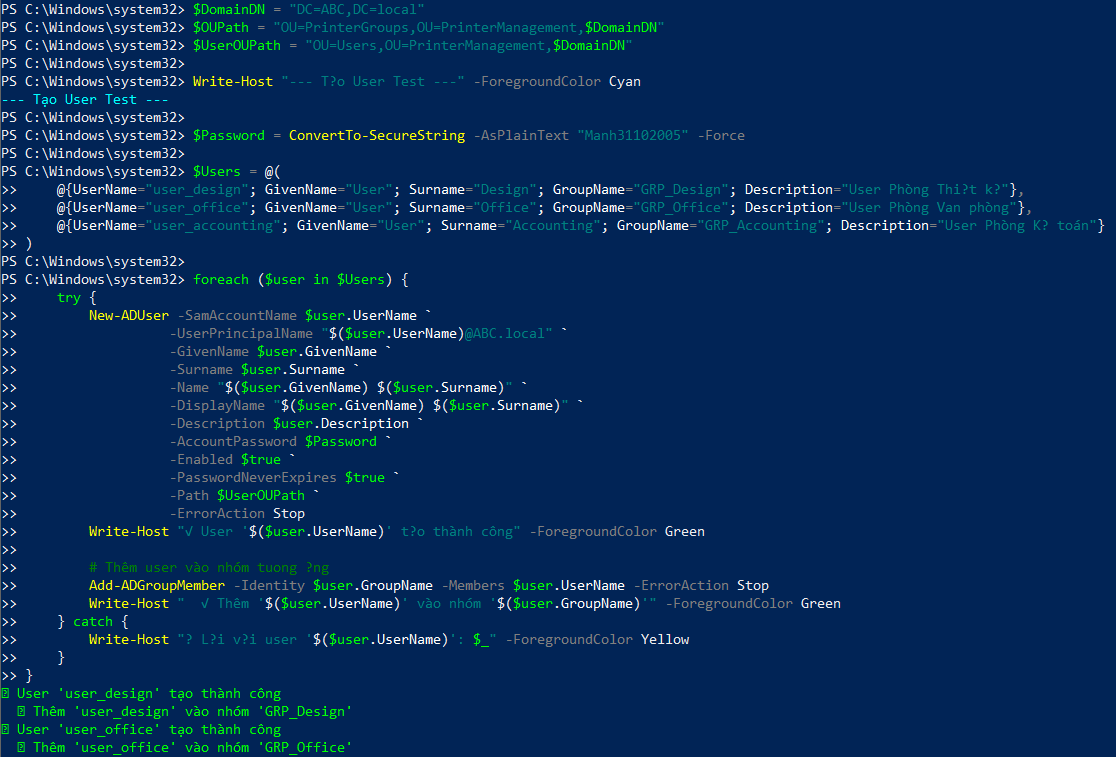
\includegraphics[width=0.78\textwidth]{./media/Tạo Nhóm AD cho từng phòng ban.png}
    \caption{Tạo Nhóm AD và thêm các User vào từng phòng ban}
    \label{fig:users_groups}
\end{figure}
\vspace{\baselineskip}

\chapter{\textbf{Triển khai Port và Driver}}
\section{Tạo TCP/IP port cho máy in}

\begin{lstlisting}[style=powershell]
Write-Host "=== Create TCP/IP Printer Ports ===" -ForegroundColor Cyan

$PrinterIPRange = 201..210

foreach ($i in $PrinterIPRange) {
    $IP = "192.168.244.$i" 
    $PortName = "IP_192.168.244.$i"
    
    try {
        Add-PrinterPort -Name $PortName `
            -PrinterHostAddress $IP `
            -ErrorAction Stop
            
        Write-Host "[OK] Printer port '$PortName' ($IP) created successfully" -ForegroundColor Green
    } catch {
        if ($_ -like "*already exists*") {
            Write-Host "[!] Port '$PortName' already exists" -ForegroundColor Yellow
        } else {
            Write-Host "[!] Error with port '$PortName': $_" -ForegroundColor Yellow
        }
    }
}

# Check port list
Write-Host "`n=== Printer Port List ===" -ForegroundColor Cyan

Get-PrinterPort | Where-Object {$_.Name -like "IP_192.168.244.*"} | Select-Object Name, PrinterHostAddress | Format-Table -AutoSize
\end{lstlisting}

\begin{figure}[htbp]
    \centering
    \begin{minipage}[b]{0.48\textwidth}
        \centering
        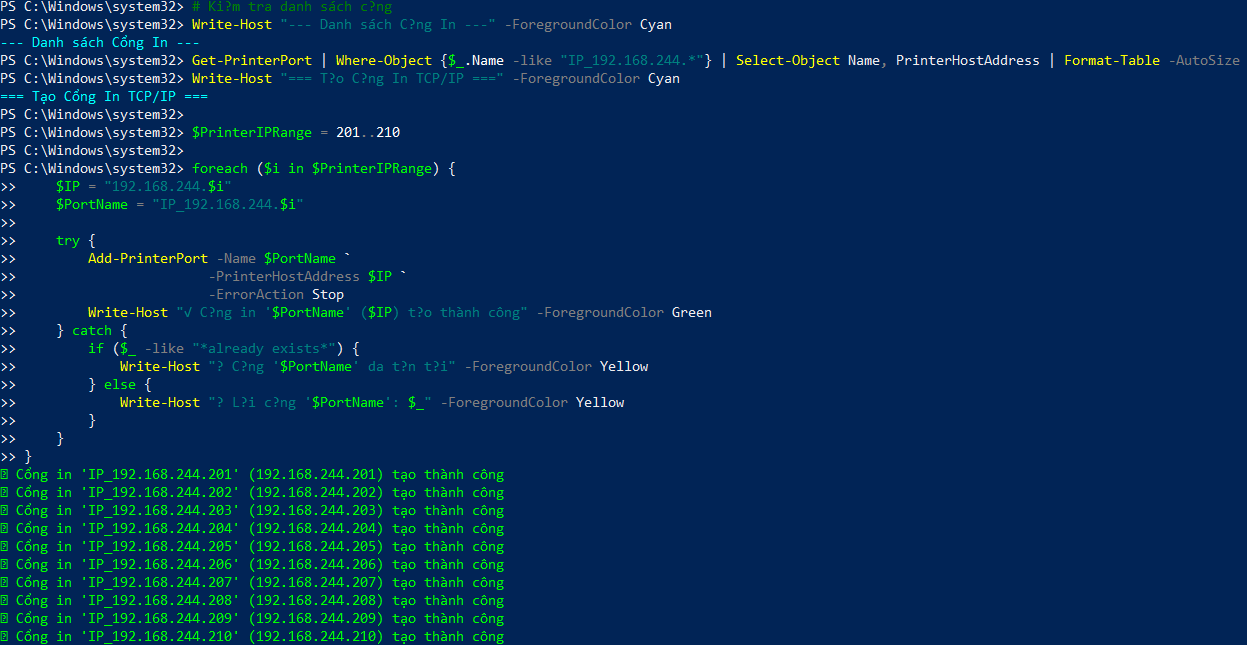
\includegraphics[width=\textwidth]{./media/TẠO CÁC CỔNG IN (PORTS).png}
        \caption{Tạo các cổng Port để in (1)}
        \label{fig:ports1}
    \end{minipage}
    \hfill
    \begin{minipage}[b]{0.48\textwidth}
        \centering
        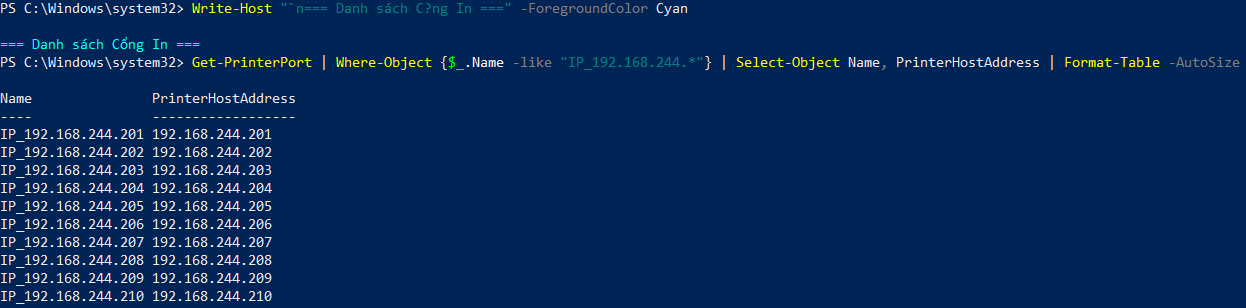
\includegraphics[width=\textwidth]{./media/TẠO CÁC CỔNG IN (PORTS)(1).png}
        \caption{Tạo các cổng Port để in (2)}
        \label{fig:ports2}
    \end{minipage}
\end{figure}

\section{Kiểm tra và cài driver}
\subsection{Cài đặt HP Universal Print Driver PCL6 64-bit}

\noindent\textbf{Lý do chọn HP Universal Print Driver PCL6 64-bit:}

\begin{itemize}[leftmargin=*,noitemsep,topsep=3pt]
    \item \textbf{Phù hợp môi trường doanh nghiệp:} Driver Universal của HP (PCL6) hỗ trợ nhiều model máy in HP khác nhau, giúp triển khai máy in cho nhiều phòng ban mà không cần cài từng loại driver riêng biệt.
    \item \textbf{Tương thích với nhiều thiết bị:} HP UPD được thiết kế để hoạt động ổn định với phần lớn các máy in HP, phù hợp với lab kiểu doanh nghiệp có nhiều máy in.
    \item \textbf{Hỗ trợ chuẩn in phổ biến:} PCL6 là ngôn ngữ in tiêu chuẩn, giúp chia sẻ tài nguyên và tạo pool máy in ảo dễ dàng.
    \item \textbf{Dễ dàng triển khai tự động hóa:} Driver universal đơn giản hóa cấu hình, phân phối qua PowerShell, Group Policy (GPO).
    \item \textbf{Tăng tính thực tế:} Dùng driver universal cho nhiều phòng ban, phân quyền, chia pool, theo dõi log phù hợp với vận hành doanh nghiệp thực tế.
    \item \textbf{Tiết kiệm thời gian:} Không lo lỗi tương thích khi cập nhật driver hoặc di chuyển máy in.
\end{itemize}

\begin{lstlisting}[style=powershell]
$driverPath = "C:\PrinterDrivers\HP-PCL6"
\end{lstlisting}

\noindent\textbf{Tìm file .INF chính:}

\begin{lstlisting}[style=powershell]
Write-Host "`n[STEP 1] Finding main .INF file..." -ForegroundColor Yellow

$allInfFiles = Get-ChildItem -Path $driverPath -Filter "*.inf" -Recurse

Write-Host "All .INF files:" -ForegroundColor Cyan
$infList = @()

for ($i = 0; $i -lt $allInfFiles.Count; $i++) {
    $inf = $allInfFiles[$i]
    $size = $inf.Length / 1KB
    
    Write-Host " [$i] $($inf.Name) ($([Math]::Round($size, 2)) KB) - Path: $($inf.Directory.Name)" -ForegroundColor Gray
    $infList += $inf
}

$rootInfs = Get-ChildItem -Path $driverPath -MaxDepth 1 -Filter "*.inf" -ErrorAction SilentlyContinue

if ($rootInfs) {
    Write-Host "`n[OK] Found .INF file in root folder:" -ForegroundColor Green
    foreach ($inf in $rootInfs) {
        Write-Host " > $($inf.Name)" -ForegroundColor Green
    }
    $mainInf = $rootInfs[0]
} else {
    Write-Host "`n[INFO] .INF file is in a subdirectory, selecting the largest file..." -ForegroundColor Yellow
    
    $mainInf = $allInfFiles | Sort-Object Length -Descending | Select-Object -First 1
    Write-Host " > $($mainInf.Name)" -ForegroundColor Cyan
}

Write-Host "`n[OK] Main .INF file used: $($mainInf.FullName)" -ForegroundColor Green
\end{lstlisting}

\begin{figure}[htbp]
    \centering
    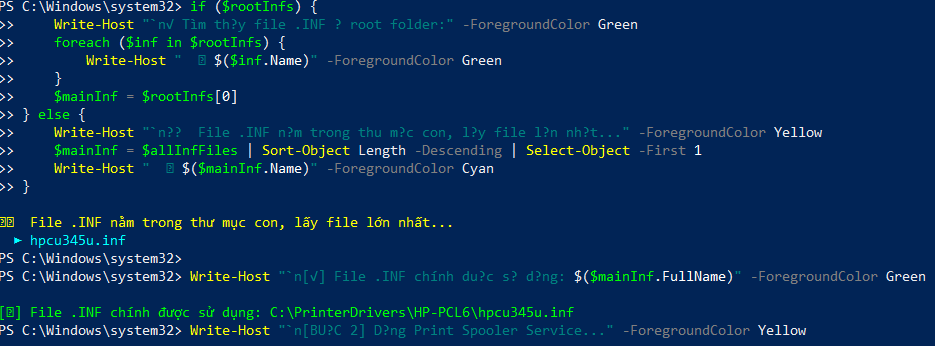
\includegraphics[width=0.78\textwidth]{./media/Tìm file .INF chính.png}
    \caption{Tìm file .INF chính}
    \label{fig:inf_file}
\end{figure}

\noindent\textbf{Dừng Print Spool:}

\begin{lstlisting}[style=powershell]
Write-Host "`n[STEP 2] Stop Print Spooler Service..." -ForegroundColor Yellow

$spooler = Get-Service -Name "Spooler"

if ($spooler.Status -eq "Running") {
    Write-Host "[STOP] Stopping Spooler..." -ForegroundColor Yellow
    Stop-Service -Name "Spooler" -Force
    Start-Sleep -Seconds 3
    Write-Host "[OK] Spooler stopped" -ForegroundColor Green
}
\end{lstlisting}

\begin{figure}[htbp]
    \centering
    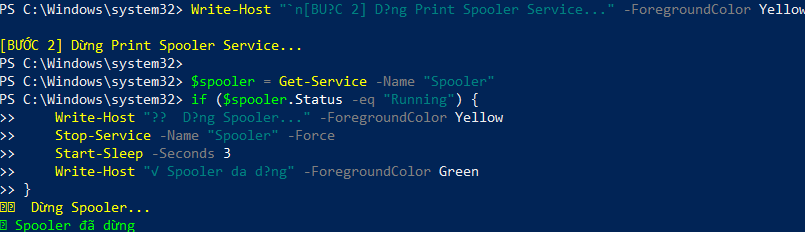
\includegraphics[width=0.78\textwidth]{./media/Dừng Print Spool.png}
    \caption{Dừng Print Spool}
    \label{fig:stop_spool}
\end{figure}

\noindent\textbf{Cài Driver bằng PNPUTIL:}

\begin{lstlisting}[style=powershell]
Write-Host "`n[STEP 3] Installing driver using pnputil..." -ForegroundColor Yellow
Write-Host " > INF File: $($mainInf.Name)" -ForegroundColor Cyan
Write-Host " > Path: $($mainInf.FullName)" -ForegroundColor Cyan
 
# Install driver from main .INF file
Write-Host "`n [*] Installing driver..." -ForegroundColor Cyan

$installOutput = & pnputil.exe -i -a "$($mainInf.FullName)" 2>&1
 
Write-Host "`n [Output from pnputil]:" -ForegroundColor Gray
$installOutput | ForEach-Object { Write-Host "    $($_.ToString())" -ForegroundColor Gray }
 
Write-Host "`n[OK] Installation command executed" -ForegroundColor Green
\end{lstlisting}

\begin{figure}[htbp]
    \centering
    \begin{minipage}[b]{0.48\textwidth}
        \centering
        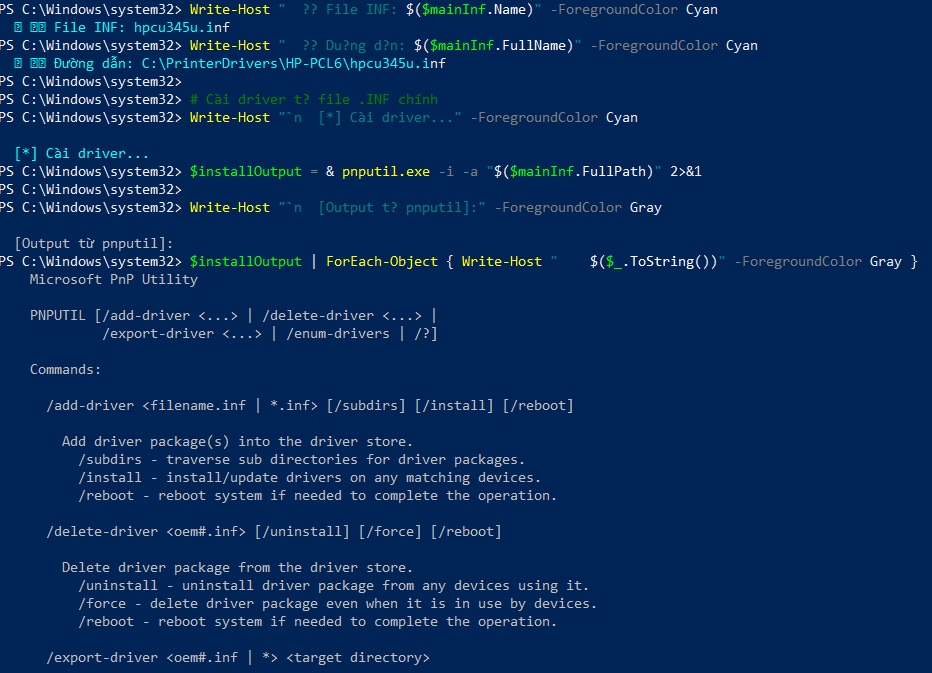
\includegraphics[width=\textwidth]{./media/Cài Driver bằng PNPUTIL.png}
        \caption{Cài Driver bằng PNPUTIL (1)}
        \label{fig:pnputil1}
    \end{minipage}
    \hfill
    \begin{minipage}[b]{0.48\textwidth}
        \centering
        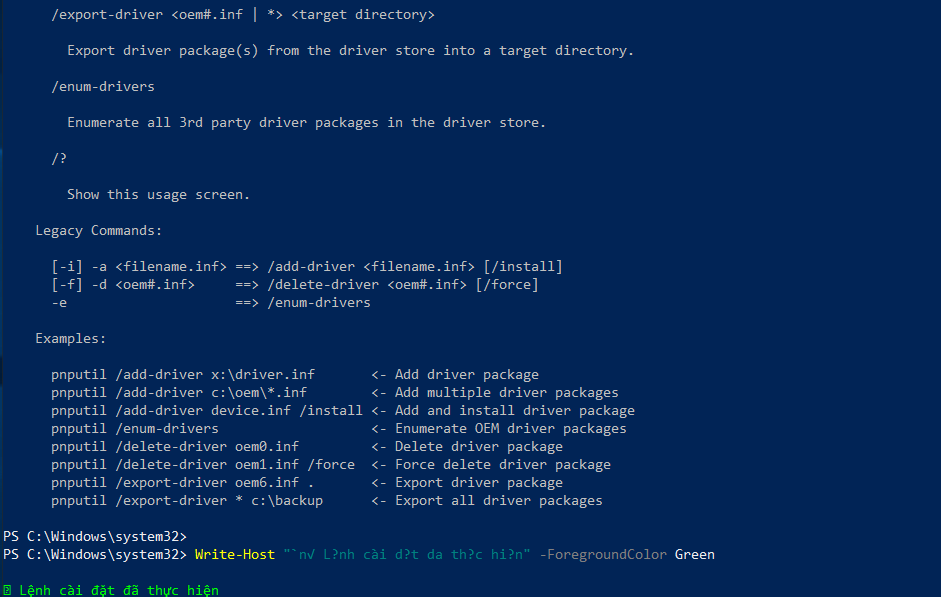
\includegraphics[width=\textwidth]{./media/Cài Driver bằng PNPUTIL(1).png}
        \caption{Cài Driver bằng PNPUTIL (2)}
        \label{fig:pnputil2}
    \end{minipage}
\end{figure}

\noindent\textbf{Khởi động lại Print Spool:}

\begin{lstlisting}[style=powershell]
Write-Host "`n[STEP 4] Restart Print Spooler..." -ForegroundColor Yellow

Start-Service -Name "Spooler"
Start-Sleep -Seconds 5

$spoolerStatus = (Get-Service -Name "Spooler").Status
Write-Host "[OK] Spooler Status: $spoolerStatus" -ForegroundColor Green
\end{lstlisting}

\begin{figure}[htbp]
    \centering
    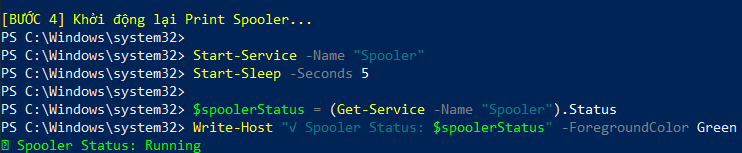
\includegraphics[width=0.78\textwidth]{./media/Khởi động lại Print Spool.png}
    \caption{Khởi động lại Print Spool}
    \label{fig:restart_spool}
\end{figure}

\noindent\textbf{Kiểm tra driver đã được cài đặt:}

\begin{lstlisting}[style=powershell]
Write-Host "`n[STEP 5] Checking installed drivers..." -ForegroundColor Yellow
 
$drivers = Get-PrinterDriver
 
if ($drivers.Count -eq 0) {
    Write-Host "[!] No drivers found!" -ForegroundColor Red
} else {
    Write-Host "`n=== PRINTER DRIVER LIST ===" -ForegroundColor Green
    
    $drivers | Select-Object @{Name="No.";Expression={$drivers.IndexOf($_)+1}}, Name, Version, PrinterEnvironment | Format-Table -AutoSize
 
    # Find HP driver
    $hpDriver = $drivers | Where-Object {$_.Name -like "*HP*" -or $_.Name -like "*Universal*" -or $_.Name -like "*PCL*"}
    
    if ($hpDriver) {
        Write-Host "`n[OK] HP DRIVER FOUND" -ForegroundColor Green
        Write-Host " Driver Name: $($hpDriver.Name)" -ForegroundColor Green
        Write-Host " Version: $($hpDriver.Version)" -ForegroundColor Green
        Write-Host " Environment: $($hpDriver.PrinterEnvironment)" -ForegroundColor Green
    } else {
        Write-Host "`n[!] HP driver not found, but other drivers exist:" -ForegroundColor Yellow
        $drivers | Select-Object Name | Format-Table -AutoSize
    }
}
\end{lstlisting}

\begin{figure}[htbp]
    \centering
    \begin{minipage}[b]{0.48\textwidth}
        \centering
        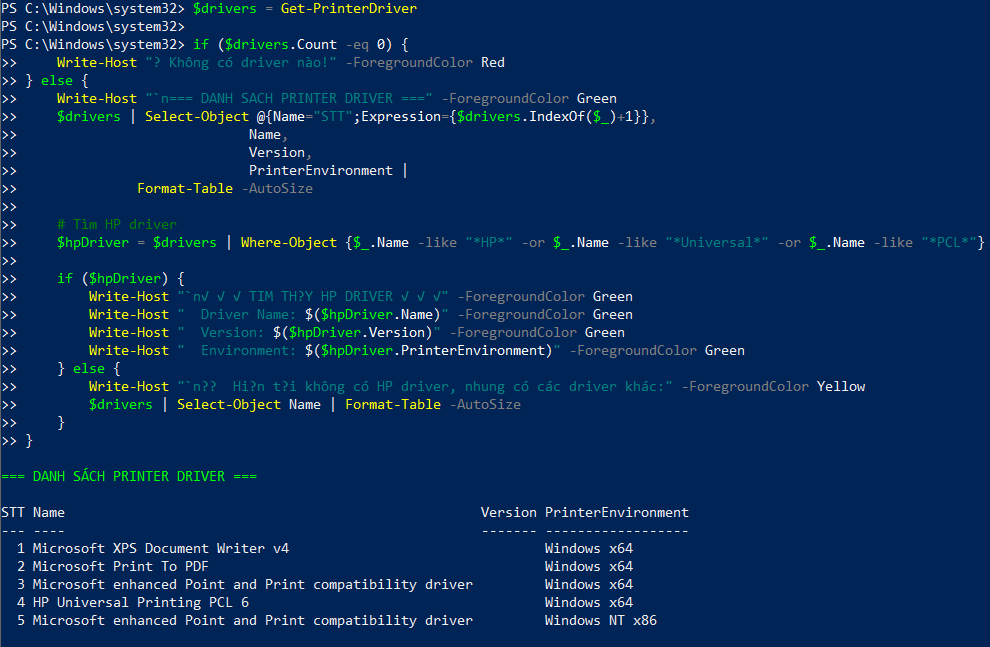
\includegraphics[width=\textwidth]{./media/Kiểm tra driver đã được cài đặt.png}
        \caption{Kiểm tra driver (1)}
        \label{fig:check_driver1}
    \end{minipage}
    \hfill
    \begin{minipage}[b]{0.48\textwidth}
        \centering
        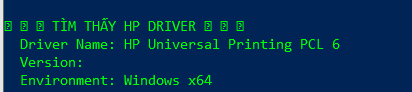
\includegraphics[width=\textwidth]{./media/Kiểm tra driver đã được cài đặt(1).png}
        \caption{Kiểm tra driver (2)}
        \label{fig:check_driver2}
    \end{minipage}
\end{figure}
\vspace{\baselineskip}

\chapter{\textbf{Tạo máy in theo từng phòng ban}}
\section{Add Printer tương ứng cho từng phòng ban}

\begin{lstlisting}[style=powershell]
Write-Host "`n=== BUOC 7: Tao May In Chia Se ===" -ForegroundColor Cyan

# Kiem tra driver co san
$AvailableDriver = Get-PrinterDriver -Name $DriverName -ErrorAction SilentlyContinue

if (-not $AvailableDriver) {
    Write-Host "[!] Driver '$DriverName' khong tim thay" -ForegroundColor Yellow
    $DriverName = "Generic / Text Only"
    Write-Host "Su dung driver thay the: $DriverName" -ForegroundColor Cyan
}

# Tao 10 may in don le
Write-Host "`n--- Tao 10 May In ---" -ForegroundColor Cyan

$PrinterInfo = @(
    @{Name="PRN_Design_01"; Description="May in Mau - Phong Thiet ke 1"; IP="192.168.244.201"; Department="Design"; Location="Tang 3, Phong Thiet ke"},
    @{Name="PRN_Design_02"; Description="May in Mau - Phong Thiet ke 2"; IP="192.168.244.202"; Department="Design"; Location="Tang 3, Phong Thiet ke"},
    @{Name="PRN_Office_01"; Description="May in B/W - Van phong 1"; IP="192.168.244.203"; Department="Office"; Location="Tang 2, Phong Van phong"},
    @{Name="PRN_Office_02"; Description="May in B/W - Van phong 2"; IP="192.168.244.204"; Department="Office"; Location="Tang 2, Phong Van phong"},
    @{Name="PRN_Office_03"; Description="May in B/W - Van phong 3"; IP="192.168.244.205"; Department="Office"; Location="Tang 2, Phong Van phong"},
    @{Name="PRN_Accounting_01"; Description="May in Hoa don - Ke toan 1"; IP="192.168.244.206"; Department="Accounting"; Location="Tang 1, Phong Ke toan"},
    @{Name="PRN_Accounting_02"; Description="May in Hoa don - Ke toan 2"; IP="192.168.244.207"; Department="Accounting"; Location="Tang 1, Phong Ke toan"},
    @{Name="PRN_Reserve_01"; Description="May in Du phong 1"; IP="192.168.244.208"; Department="Reserve"; Location="Tang 1, Phong May"},
    @{Name="PRN_Reserve_02"; Description="May in Du phong 2"; IP="192.168.244.209"; Department="Reserve"; Location="Tang 1, Phong May"},
    @{Name="PRN_Test_01"; Description="May in Test"; IP="192.168.244.210"; Department="Test"; Location="Tang 1, IT"}
)

foreach ($printer in $PrinterInfo) {
    $PortName = "IP_$($printer.IP)"
    
    try {
        Add-Printer -Name $printer.Name `
                   -DriverName $DriverName `
                   -PortName $PortName `
                   -ErrorAction Stop
        
        # Chia se may in
        Set-Printer -Name $printer.Name -Shared $true -ErrorAction SilentlyContinue
        
        Write-Host "[OK] May in '$($printer.Name)' tao thanh cong" -ForegroundColor Green
    } catch {
        Write-Host "[!] May in '$($printer.Name)' loi: $_" -ForegroundColor Yellow
    }
}

# Kiem tra danh sach may in
Write-Host "`n--- Danh sach May In Chia Se ---" -ForegroundColor Cyan
Get-Printer | Select-Object Name, Description, Location, Shared | Format-Table -AutoSize
\end{lstlisting}

\begin{figure}[htbp]
    \centering
    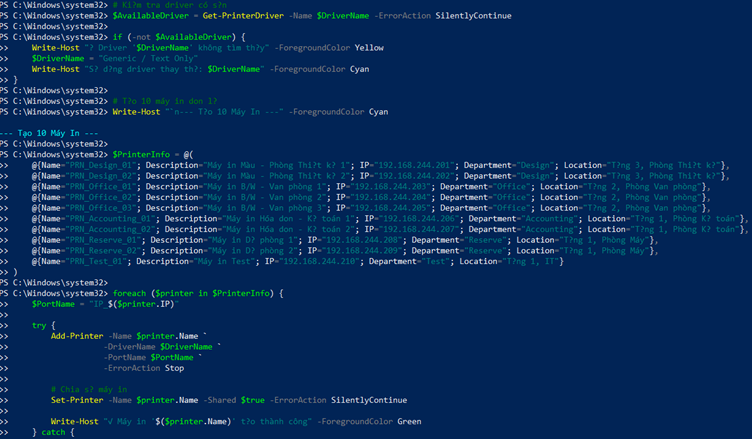
\includegraphics[width=0.78\textwidth]{./media/DS may in.png}
    \caption{Kiểm tra danh sách máy in đã tạo}
    \label{fig:printer_list}
\end{figure}

\section{Tạo Printer Pool khi cần}

\begin{lstlisting}[style=powershell]
$DriverName = "HP Universal Printing PCL 6"
$PoolName = "PRN_Pool_Office"
$PoolPrinterList = @("PRN_Office_01", "PRN_Office_02", "PRN_Office_03")
 
# Get ports from printers in the pool list
$PoolPorts = @()
foreach ($prn in $PoolPrinterList) {
    $Port = (Get-Printer -Name $prn -ErrorAction SilentlyContinue).PortName
    if ($Port) {
        $PoolPorts += $Port
    }
}
 
Write-Host "Found $($PoolPorts.Count) ports for the pool" -ForegroundColor Cyan
 
if ($PoolPorts.Count -ge 2) {
    try {
        # Create Printer Pool (Basic creation with first port)
        Add-Printer -Name $PoolName `
                   -DriverName $DriverName `
                   -PortName $PoolPorts[0] `
                   -ErrorAction Stop
        
        # Share the printer
        Set-Printer -Name $PoolName -Shared $true
        
        # OPTIONAL: Uncomment the line below to actually enable Pooling across all found ports
        # Set-Printer -Name $PoolName -PortName ($PoolPorts -join ",")

        Write-Host "[OK] Pool '$PoolName' created successfully" -ForegroundColor Green
        Write-Host " Ports in pool:" -ForegroundColor Cyan
        foreach ($port in $PoolPorts) {
            Write-Host "    - $port" -ForegroundColor Cyan
        }
    } catch {
        Write-Host "[!] Error creating Pool: $_" -ForegroundColor Yellow
    }
} else {
    Write-Host "[!] Not enough printers for the pool" -ForegroundColor Yellow
}
 
# Check
Get-Printer -Name $PoolName -ErrorAction SilentlyContinue | Format-Table
\end{lstlisting}

\begin{figure}[htbp]
    \centering
    \begin{minipage}[b]{0.48\textwidth}
        \centering
        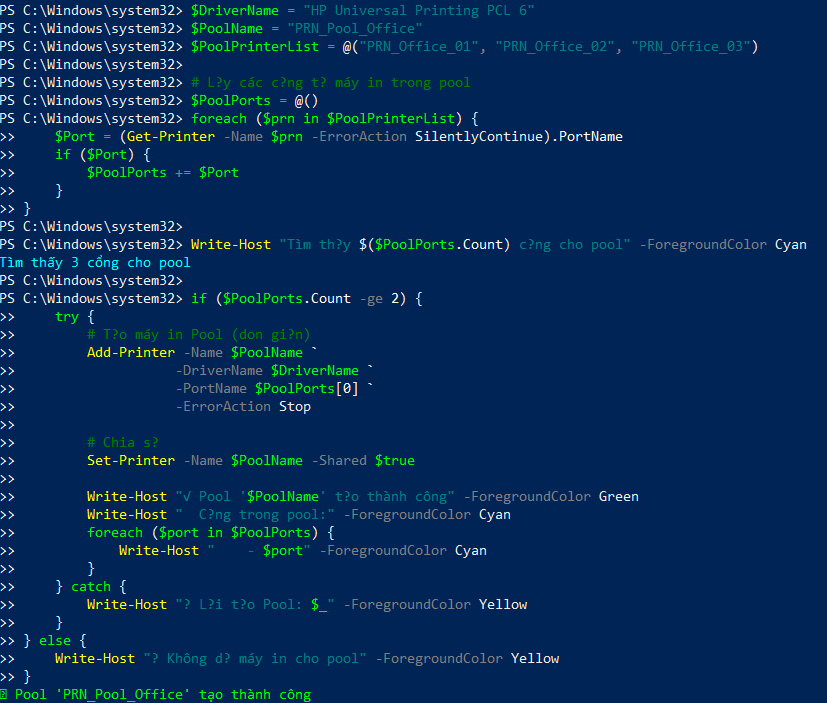
\includegraphics[width=\textwidth]{./media/TẠO PRINTER POOL CHO PHÒNG VĂN PHÒNG.png}
        \caption{Tạo Printer Pool (1)}
        \label{fig:pool1}
    \end{minipage}
    \hfill
    \begin{minipage}[b]{0.48\textwidth}
        \centering
        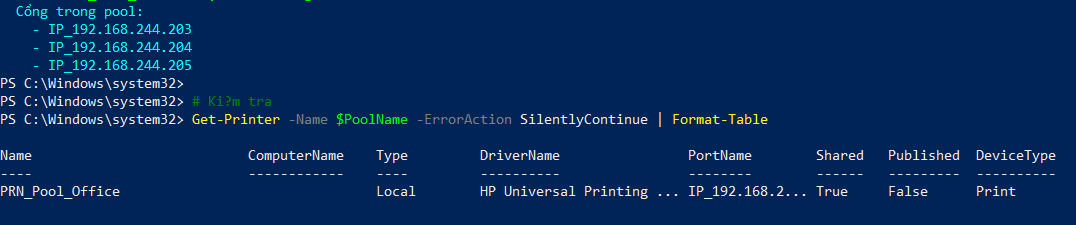
\includegraphics[width=\textwidth]{./media/TẠO PRINTER POOL CHO PHÒNG VĂN PHÒNG(1).png}
        \caption{Tạo Printer Pool (2)}
        \label{fig:pool2}
    \end{minipage}
\end{figure}